%\addcontentsline{toc}{chapter}{Development Process}
\chapter{Design}

In FDD, large, detailed design documents are not necessary. A simple overview of desired features and a breakdown of the overall system are sufficient, and are what will be detailed in this chapter.

\section{Overall Architecture}
\label{sec:des_Architecture}
As the project was developed using Feature Driven Development (FDD), the initial design of the system focused on the desired features of the system. These features were:
\begin{itemize}
	\item Download the dataset.
	\item Parse the original data into a more useful format.
	\item Allow a user to annotate the data with sentiment, to generate training and testing datasets.
	\item Train an AI algorithm on the datasets generated.
	\item Search the parsed data to find speech about a certain topic, or by a particular Member of Parliament.
	\item Use the trained AI algorithm to extract sentiment from the speech found.
	\item Display a comparison of the sentiment expressed about a topic or by an MP over time.
\end{itemize}

Using these features, the overall system can be designed, and an unofficial class diagram can be created that can help guide implementation.

\begin{figure}[ht]
	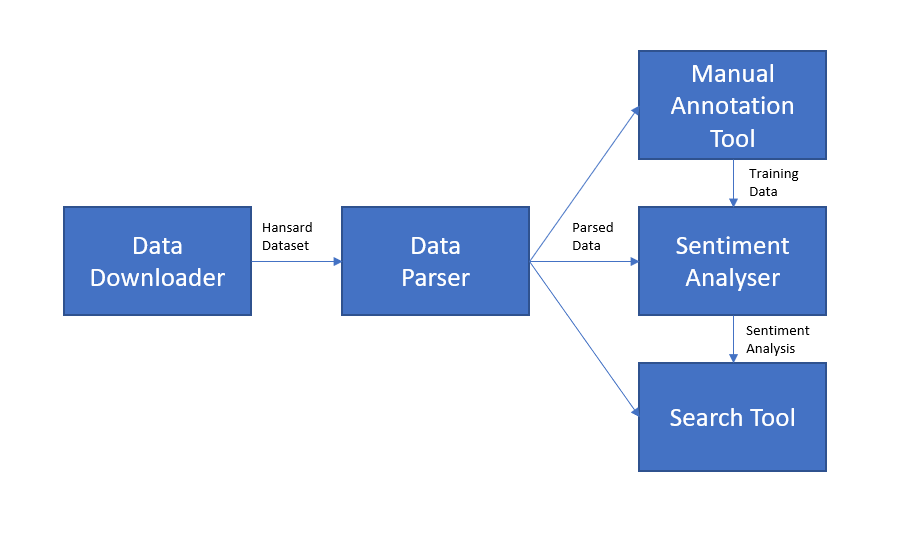
\includegraphics[width=\textwidth]{project_block_diagram}
	\caption{Functional block diagram of the overall system. Arrows represents data movement}
	\label{fig:project_block_diagram}
\end{figure}

As seen in fig.\ref{fig:project_block_diagram}, the system is broken down into functional blocks, each representing a distinct part of the system. They were split this way to maintain readability in the source code. Whilst it would have been possible to keep all functionality in a single file, it would have made maintaining the code very difficult. Each functional block is therefore a separate class in the Python source code, so any interaction between them is easy to manage.

\subsection{Data Downloader}
\label{sec:des_data_downloader}
The Data Downloader is designed to download all of the Hansard Dataset from the site on-line, and store it locally for use by the rest of the system. It is likely that this first block will only need to be run a single time, but still proves useful in ensuring all the data is downloaded.

The files are to be downloaded from the \href{http://www.hansard-archive.parliament.uk}{Hansard Archive} page. Each of the six series has a subdirectory under that root page, that contain all the data files. The data files have a distinct naming pattern that can be referenced using something like Regular Expressions in order to automate the downloading and searching of the files.

Originally, this was not going to be a part of the main system, as it is possible to download the data manually. However, only ten files are displayed on the web page each time, and some of the series have up to a thousand files to download. This can be seen in fig.\ref{fig:Archive_Screenshot}

\begin{figure}[ht]
	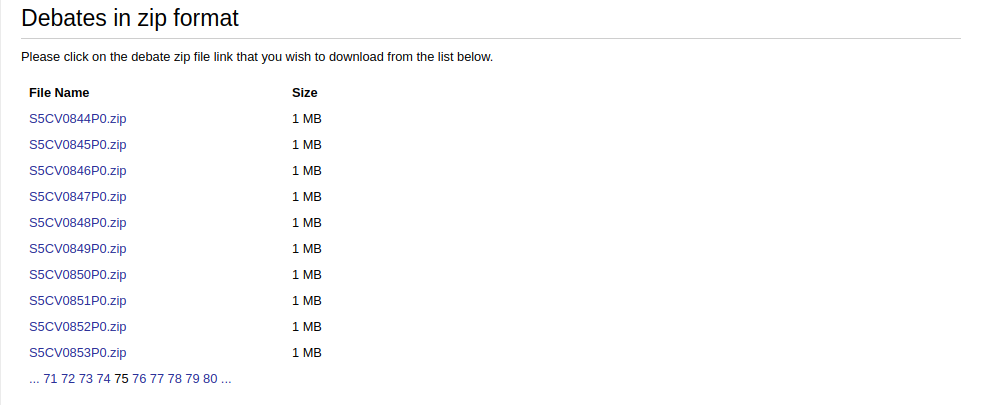
\includegraphics[width=\textwidth]{archive_screenshot}
	\caption{Screen capture from the Hansard Archive website, showing the number of files available}
	\label{fig:Archive_Screenshot}
\end{figure}

\subsection{Data Parser}
\label{sec:des_data_parser}
The Parser is designed to read the original files downloaded by the Data Downloader, and save all relevant data in separate location, in a more consistent layout than that of the original dataset. This should allow any usage of the data from other parts of the system to be much simpler, and thus faster and less prone to error. It should ensure speech is always attributed to the correct person, even if their names are presented differently. This means the Data Parser will have to utilize a part of NLP known as Name Disambiguation, which is not a simple task. 

\subsection{Manual Annotation Tool}
\label{sec:des_annotation_tool}
The Manual Annotation Tool (the MAT) is designed to allow a user to create a testing and training dataset from the parsed data. It should show a selection of speech to the user, and ask them to annotate it as either a positive sentiment, negative sentiment, or neutral sentiment. These choices will be recorded, and can then be used to train a machine learning algorithm to extract sentiment from the remaining data. It would also provide the option to edit the text, the MP's name, or the topic title, to allow the user to correct typos transfered from the original dataset.

Originally, the MAT would display an entire paragraph of speech, displaying everything a Member of Parliament said about a topic on a particular day. However, this would often display too much text, with parts showing positive sentiment and other parts of the same text showing negative sentiment. Additionally it was realized that attempting to train an AI algorithm on these large blocks of text would be far too complex. For those reasons, the MAT was modified so that it would only display a single sentence at a time, allowing a more accurate way of annotating sentiment.

\subsection{Sentiment Analyzer}
\label{sec:des_sentiment_analyzer}
The Sentiment Analyzer will use the datasets generated by the MAT and produce a model based off the data. It should also provide the ability to load a previously trained model, rather than spend time retraining every time the system is run. Once trained or loaded, it should be able to accept blocks of text, which it can then extract sentiment from, and return it.

As AI algorithms are trained on "Features" rather than plain text, the Sentiment Analyzer must have some method of converting a sentence or paragraph into a set of features for the algorithm to use. Following on from a tutorial found on Youtube \cite{NLTKYoutubePlaylist}, it appears that a good way to turn the text into a set of features is to use a dictionary, where the keys are the most used words from the training set, and the value is a True or False, for if the word is contained in the sentence or paragraph given. The potential issue with this is the loss of context, as separating the words completely will lose any negation, such as in the sentence "This is not good".

\subsection{Search Tool}
\label{sec:des_search_tool}
The Search Tool will be used by the user to search through the data for a particular Member of parliament, to get their speech and its sentiment, or for a particular topic, to get the sentiment expressed about that topic. 

\section{Data Design}
\label{sec:des_data}
As parts of the system were designed to modify the layout of the original data at times, the formatting of said data had to be designed as well.

\subsection{Parsed Data}
\label{sec:des_parsed_data}
For the parser, the format of the data files that it produces was originally designed as thus:
\begin{lstlisting}[language=XML]
<date dateformat="1984/04/13">	
    <speech>
        <member>memberName</member>
        <topic>topicTitle</topic>
        <stance>POS/NEG</stance>
        "Actual Text of Speech would go Here"
    </speech>
    ....
</date>
....
\end{lstlisting}
The ellipses represent repeats, so inside the \emph{Date} tags, multiple \emph{speech} tags, all formatted like the one shown, can exist. A file may also contain multiple \emph{Date} tags. 

This, however, was causing some issues during development based around the size of the produced files, as each entire series of data was being parsed into the same file. In order to combat the slow speeds of accessing such large files, and other issues caused by the layout, the data format was changed. Now, each unique date found within the source had a separate file, and within this file the data was formatted in its final form.
Each date file is an XML file, the structure of which can be represented as a tree, shown in fig.\ref{fig:parsed_data_tree}.

\begin{figure}[ht]
	\includegraphics[width=\textwidth]{parsed_data_tree}
	\caption{Diagram showing the structure of the parsed data, in XML. The \emph{Date} tag is the root of the file}
	\label{fig:parsed_data_tree}
\end{figure}

Each file can contain multiple member tags, which each have the member of parliament’s name as an attribute. Each member tag can contain multiple tags for the topics they discuss, each of which have the topic title as an attribute. Each topic tag can have multiple speech tags, each speech tag containing the verbatim copy of what the member said about the particular topic.

\subsection{Annotated Data}
\label{sec:des_anotate_data}
The formatting of the annotated data files was also designed at this stage. It was decided that the files would be saved as CSV files (comma separated values), which is a simplistic database style where a line in the file represents a single record, each value of the record being separated by a comma, hence the name. The layout was designed as the following:

\textbf{Sentence; Sentiment; Member; Topic}

As shown, it was decided that the best way of annotating full speech was to split it by sentence, so that each sentence would be annotated with its own sentiment. This would simplify the training process for the machine learning algorithms, as it was thought that trying to train it on too large a block of text would result in sub par results.

\section{User Interface}
\label{sec:des_user_interface}
Due to the complexity of the project, it was decided that the system would only be interacted with via the command line. This meant that, beyond basic menus, no GUI had to be designed for use. It was though that, should there be time during or after the project development, a GUI could be designed which worked by interacting with the command line interface in the background, but it was not considered system critical to have such a thing.

\section{Algorithm Design}
\label{sec:des_algorithm}

\subsection{AI Algorithm Choice}
\label{sec:des_AI_algorithm}
There are many potential algorithms that may be chosen for this project. It may prove difficult to choose one, or more, without simply trying them. The design calls for the use of Naive Bayes at first, mainly as its one provided by the NLTK package. However, multiple other algorithms may be tested, and the results compared to decide on the final choice. Should multiple algorithms prove useful, a voting system could be implemented, which applies each algorithm, and they cast a vote to what sentiment they "think" applies. The votes would then be counted and the result shown.

\subparagraph{Naive Bayes}
Naives Bayes is a supervised algorithm with uses the statistical analysis of Bayes Theorem as to classify data. It treats each feature as completely distinct, which isn't accurate for NLP, but will may suffice for development of the system.

\subsection{Parsing}
\label{sec:des_Parsing_algorithm}
The Data Parser needs to find and extract useful speech from the original data. Though said data is somewhat disorganized, there are exploitable patterns that the Parser can use to find as much speech as possible. The overall method is documented in the following pseudo-code:
\begin{lstlisting}
FOR EACH FILE
    FOR EACH DATE TAG
    	IF(DATE_FILE FOR DATE EXISTS)
        	LOAD DATE_FILE CONTENTS INTO DATE_XML
    	ELSE
        	CREATE FILE
        	CREATE DATE_XML
    	FOR EACH CONTRIBUTION IN DATE_TAG
        	GET CONTRIBUTION PARENT_TAG
        	GET MEMBER NAME AS CHILD OF PARENT_TAG
        	GET TITLE AS SIBLING OF PARENT_TAG
        	GET SPEECH FROM CONTRIBUTION
        	IF MEMBER HAS BEEN SEEN BEFORE IN CURRENT DATE_FILE
        	    IF TOPIC HAS BEEN DISCUSSED BY MEMBER BEFORE
        			ADD SPEECH TO TOPIC
        		ELSE
        			CREATE NEW TOPIC
        			ADD SPEECH
        	ELSE
        		CREATE NEW MEMBER TAG
        		ADD TOPIC TO MEMBER TAG
        		ADD SPEECH TO TOPIC
        	ADD SPEECH TO DATE_XML

    SAVE XML TO DATE_FILE (OVERWRITE)
\end{lstlisting}

This shows that, so long as the parser can find a tag in the source XML for the date, all other relevant information can be found in relation to the position of this date tag in the XML. It also shows the method of ensuring all speech by one Member of Parliament is correclty attributed to them, to avoid repeated mentions of the same MP in the same file.